% 4-1 题 图4_1：质量m小球水平朝右速度v，相对矩形中A,B,C三顶点
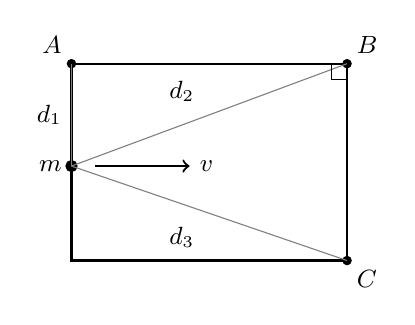
\begin{tikzpicture}[font=\small]
  % 长方形
  \draw[thick] (0,2.5) -- (3.5,2.5) -- (3.5,0) -- (0,0) -- cycle;
  % 顶点标注
  \filldraw (0,2.5) circle (1.5pt) node[above left] {$A$};
  \filldraw (3.5,2.5) circle (1.5pt) node[above right] {$B$};
  \filldraw (3.5,0) circle (1.5pt) node[below right] {$C$};
  % 小球位置（在矩形左侧边的某处）
  \filldraw (0,1.2) circle (2pt) node[left] {$m$};
  % 速度箭头（水平朝右）
  \draw[->, thick] (0.3,1.2) -- (1.5,1.2) node[right] {$v$};
  % 标注各距离
  \draw[thin, gray] (0,1.2) -- (0,2.5);
  \node[left] at (0,1.85) {$d_1$};
  \draw[thin, gray] (0,1.2) -- (3.5,2.5);
  \node[above, sloped] at (1.4,1.9) {$d_2$};
  \draw[thin, gray] (0,1.2) -- (3.5,0);
  \node[below, sloped] at (1.4,0.55) {$d_3$};
  % 直角符号在B处
  \draw (3.3,2.5) -- (3.3,2.3) -- (3.5,2.3);
\end{tikzpicture}
